\documentclass[12pt]{article}
\usepackage[utf8]{inputenc}
\usepackage[paper=letterpaper,margin=2cm]{geometry}
\usepackage{amsmath}
\usepackage{amsthm}
\usepackage{amssymb}
\usepackage{amsfonts}
\usepackage{enumitem}
\usepackage{titling}
\usepackage[spanish]{babel}
\decimalpoint
\usepackage[colorlinks=true]{hyperref}
\usepackage{listingsutf8}
\usepackage[pdftex]{graphicx}
\usepackage{caption}
\usepackage{subcaption}
\usepackage{fancyhdr}
\usepackage{multirow}
\usepackage{biblatex}
\usepackage{physics}
\usepackage{siunitx}
\usepackage{color}
\usepackage{tikz}

%\usepackage[table,xcdraw,dvipsnames]{xcolor}
\usepackage{xcolor}
\usepackage{tocloft}
\addbibresource{ref.bib}
\hypersetup{linkcolor=blue}
\newcommand{\m}{\text{m}}
\newcommand{\mpers}{\unit[per-mode = symbol]{\metre\per\second}}
\definecolor{codegreen}{rgb}{0,0.5,0}
\pagestyle{fancy}
\fancyhf{}

\title{Plantilla prácticas}
\author{Rodrigo Rafael Castillo Chong}
\date{\today}
\begin{document}
\lstset{inputencoding=utf8/latin1}
\lstdefinestyle{myStyle}{
	keywordstyle=\color{blue},
	commentstyle=\color{codegreen},
	backgroundcolor=\color{gray!10!white},
}
\lstset{style=myStyle}
	\thispagestyle{empty}
	
	\begin{figure}[ht]
		\minipage{0.7\textwidth}
		
\includegraphics[width=4cm]{images/usaclogo.png}
		\label{EscudoUSAC}
		\endminipage
		\minipage{0.32\textwidth}
		
\includegraphics[height = 4cm ,width=4cm]{images/logoecfmplain.png}
		\label{EscudoECFM}
		\endminipage
	\end{figure}
	
	\begin{center}
		\vspace{0.8cm}
		\LARGE
		UNIVERSIDAD DE SAN CARLOS DE GUATEMALA
		
		\vspace{0.8cm}
		\LARGE
		ESCUELA DE CIENCIAS FÍSICAS Y MATEMÁTICAS
		
		\vspace{1.7cm}	
		\Large
		\textbf{Informe final de prácticas}
		
		\vspace{1.7cm}
		\Large
		\textbf{Evaluación de distintos métodos numéricos para resolver ecuaciones particulares de la mecánica de fluidos}
		
		
		\vspace{1.3cm}
		\normalsize	
		POR \\
		\vspace{.3cm}
		\large
		\textbf{Rodrigo Rafael Castillo Chong \\ 201804566}
		
		\vspace{1.3cm}
		\normalsize	
		ASESORADO POR \\
		\vspace{.3cm}
		\large
		\textbf{Enrique Pazos, Ph.D.}
		
		
		
		\vspace{1.3cm}
		\today
	\end{center}
	
	\newpage
	\tableofcontents
	\clearpage
	
	\section{Método de diferencias finitas}
	El \textbf{método de diferencias finitas} o \textbf{método DF} es un método numérico que sirve para resolver ecuaciones diferenciales ordinarias o parciales. El método consiste en discretizar el dominio de la ecuación en un conjunto finito de puntos llamado \textbf{grilla}; donde cada punto debe estar a la misma distancia de cada uno de sus vecinos. Posteriormente se deben aproximar las derivadas de la función con ecuaciones de diferencias utilizando series de potencias, para poder resolver la versión aproximada de la ecuación diferencial algebraica iterativamente \cite{devries2011first}.
	
	Un ejemplo de discretización, que se usa al aplicar el método DF en una ecuación diferencial parcial, es el siguiente: la segunda derivada parcial respecto a $x$ de una función $u = u(x,t)$ valuada en $(x,t)$ se puede aproximar expandiendo la función en dos series de Taylor centradas en dos diferentes valores sobre el eje $x$, que corresponden a los dos puntos vecinos a $x$, separándose de este punto por una distancia $\Delta x$; también llamada \textbf{tamaño de paso} en $x$. 
	
	Para obtener la aproximación de la segunda derivada de $u$ respecto a $x$ se utilizan las expansiones en series de Taylor:

	\begin{equation}
		u(x + \Delta x,t) \approx u(x,t) + \Delta x\pdv{u(x,t)}{x} + \frac{(\Delta x)^{2}}{2}\pdv{^{2}u(x,t)}{x^2} 
	\end{equation}

	\begin{equation}
		u(x - \Delta x,t) \approx u(x,t) - \Delta x\pdv{u(x,t)}{x}+\frac{(\Delta x)^{2}}{2}\pdv{^{2}u(x,t)}{x^2} 
	\end{equation}
	Sumando ambas aproximaciones se obtiene:
	\begin{equation}
		(\Delta x)^2 \pdv{^{2}u(x,t)}{x^2}\approx u(x + \Delta x,t) + u(x - \Delta x,t) - 2 u(x,t)
	\end{equation}

	\begin{equation}
		\pdv{^{2}u(x,t)}{x^2}\approx \frac{u(x + \Delta x,t) + u(x - \Delta x,t) - 2 u(x,t)}{(\Delta x)^2}
	\end{equation}
	Por tanto, se puede aproximar una derivada de segundo orden en términos de valores conocidos, puesto que $u(x + \Delta x,t)$ y $u(x - \Delta x,t)$ corresponden a valores que toma la función en un dominio discretizado, en donde la distancia entre los puntos de la grilla es siempre $\Delta x$. Se puede escribir la función valuada en forma discreta:
	\[u_{i} := u(x,t)\]
	\[u_{i+1} := u(x + \Delta x,t)\]
	\[u_{i-1} := u(x - \Delta x,t)\]
	De tal forma que la aproximación de la segunda derivada parcial se puede representar de manera compacta
	\begin{equation}
		\pdv{^{2}u}{x^2} \approx \frac{u_{i+1}-2u_{i}+u_{i-1}}{(\Delta x)^{2}}
		\label{eq:segunda-derivada-discreta}
	\end{equation}
	En la figura \ref{fig:discretizacion} se observa la representación gráfica de esta discretización.
	
	\begin{figure}[ht]
		\centering
		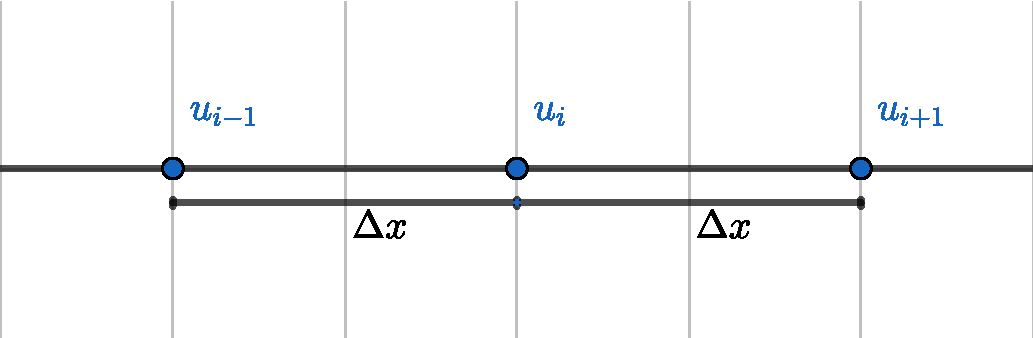
\includegraphics[scale=0.8]{images/grilla.pdf}
		\caption{Discretización del dominio espacial}
		\label{fig:discretizacion}
	\end{figure}
	
	
	En general, el dominio temporal de la función también se discretiza, tomando intervalos de tiempo consecutivos separados por un intervalo de tiempo $\Delta t$ o también llamado tamaño de paso en $t$. 
	
	\newpage
	Para aproximar la primera derivada parcial en $t$ de $u$ se expande la función en una serie de Taylor centrada en $\Delta t$ y el término donde la función está valuada en el instante temporal mayor se renombra como $u_{\text{nueva}}$.
	
	\[u(x,t+\Delta t)\approx u(x,t) + \Delta t \pdv{u(x,t)}{t}\]
	\[\pdv{u(x,t)}{t} \approx \frac{u(x,t+\Delta t) - u(x,t)}{\Delta t}\]
	\[\pdv{u(x,t)}{t} \approx \frac{u_{\text{nueva,} i} - u_{i}}{\Delta t}\]
	
	Posteriormente se reemplazan las discretizaciones aproximadas en la ecuación diferencial a resolver y se itera sobre la relación de recurrencia encontrada para los valores actuales y futuros de la función en un punto dado. 
	
	En resumen, el método DF funciona aproximando y adaptando las derivadas de primer y segundo orden a ecuaciones de diferencias que dependen de los valores que la función devuelve cuando esta se valúa en los puntos de la grilla, o bien, en instantes discretos de tiempo.\\
	
	A continuación se describen los problemas resueltos con el método de diferencias finitas y los resultados conseguidos con este.

	
	\subsection{Ecuación de Burgers no viscosa, en una dimensión}
	\label{sec:burgers1ddf}
	\subsubsection{Descripción del problema}
	La ecuación de Burgers no viscosa en una dimensión espacial es una ecuación diferencial parcial no lineal de primer orden que expresa la evolución temporal de la cantidad $u = u(x,t)$, la cual se interpreta como la componente en $x$ de la \textbf{velocidad} de un fluido o gas. La ecuación tiene la siguiente forma:
	\begin{equation}
		\pdv{u}{t}+u\pdv{u}{x}=0
		\label{eq:burgers1d}
	\end{equation}
	
	Se resolvió esta ecuación en un dominio espacial $I$ dado por $I = [0,\text{L}]$, donde $\text{L} = 100 \unit{\meter}$, y sujeta a las siguientes condiciones de frontera:\\
	\begin{equation}
		u(0,0)=0
	\end{equation}
	\begin{equation}
		u(\text{L},0)= 0
	\end{equation}
	La imposición de estas condiciones pueden interpretarse como el modelado de un fluido sin presión ni viscosidad, o un gas, que se mueve en una dimensión cuyos extremos simulan un tope o frontera que impide que el fluido o gas en cuestión salga. 
	
	Como condición inicial se eligió una distribución gaussiana de velocidad. Esta se puede interpretar como un pulso centrado en el centro del dominio. Es común utilizar pulsos gaussianos como condiciones iniciales, para así visualizar su desplazamiento a lo largo de la simulación\footnote{En las ecuaciones se mantuvieron los nombres de las variables utilizadas en el código de la integración numérica de la ecuación, salvo por $\mu$ que se escribió como \texttt{mu}.}.
	\begin{equation}
		u(x,0) = A\exp(-b(x-\mu)^{2})
		\label{eq:condinicial}
	\end{equation}
	\\
	Donde:
	\begin{itemize}
		\item $A=3.5\mpers$
		\item $b=0.05$
		\item $\mu=L/2=50\unit{\meter}$
	\end{itemize}

	\subsubsection{Aplicación del método y código implementado}
	Se utilizó el lenguaje \texttt{C++} para resolver el problema numérico utilizando el método de diferencias finitas. El código completo está disponible en el siguiente \href{https://github.com/highchen147/practicas/blob/main/burgers1DDF/burgers1DDF.cpp}{enlace.}
	
	
	Para resolver numéricamente la ecuación \ref{eq:burgers1d} utilizando el método DF, primero se debe discretizar el dominio en el que esta se define. Para la simulación se definió un conjunto de \texttt{Nx} puntos sobre el eje $x$ de tal manera que cada par de puntos vecinos estuvieran separados por una distancia \texttt{dx}, la cual equivale a $\Delta x$ en la simbología algebraica de este documento.
	
	\lstinputlisting[title = Valores de los parámetros para discretización del dominio espacial, language = C++,
	firstline=30,
	lastline=32,
	commentstyle=\color{codegreen},
	keywordstyle=\color{blue}]{../burgers1DDF/burgers1DDF.cpp}
	
	Es destacable que el denominador de la fracción que define a \texttt{dx} es $\texttt{Nx-1}$ dado que el intervalo contiene esta cantidad de veces la distancia \texttt{dx.} 

	Para almacenar los valores de la función $u$ se utilizaron punteros a arreglos dinámicos de tipo \texttt{\color{blue}{double}}, al igual que para almacenar el conjunto de puntos que conforma el dominio discretizado en el eje $x$. Estos también fueron inicializados dependiendo de su definición; en el caso de $u$, se aplicó la condición inicial del problema y las condiciones de frontera.	
	
	\lstinputlisting[title = Definición e inicialización de arreglos dinámicos, 
	language = C++, 
	firstline=42,
	lastline=61,
	keywordstyle=\color{blue}]{../burgers1DDF/burgers1DDF.cpp}
	
	\lstinputlisting[title = Implementación de la ecuación \ref{eq:condinicial}, 
	language = C++,
	firstnumber = 112,
	firstline=112,
	lastline=118,
	keywordstyle=\color{blue}]{../burgers1DDF/burgers1DDF.cpp}
		
	
	Para discretizar el dominio temporal se tomó \texttt{t\_total} como la variable que almacena el tiempo total a simular y \texttt{dt} como el tamaño de paso temporal. Por tanto, el número de iteraciones necesarias para simular el tiempo completo se obtiene dividiendo \texttt{t\_total} entre \texttt{dt}. Sin embargo, puede que el resultado de esta división no sea un número entero, por lo que se le aplica la función \texttt{floor()} para garantizarlo. La variable \texttt{num\_outs} es un número entero que indica cuántos instantes temporales serán impresos en el archivo de datos; esta cantidad es importante ya que la velocidad de simulación depende de qué tantas veces se imprimen los datos. Las variables de tipo \texttt{const} pueden ser cambiadas a voluntad del usuario, siempre y cuando el cambio sea efectuado en la declaración de las mismas.
	
	\lstinputlisting[title = Valores de los parámetros para discretización del dominio temporal, language = C++, 
	firstline=19, 
	lastline=27, 
	keywordstyle=\color{blue}]{../burgers1DDF/burgers1DDF.cpp}
	
	El siguiente paso para implementar el método consistió en aproximar las derivadas utilizando los valores disponibles sobre la grilla, esto es:
	\begin{equation}
		\pdv{u}{x} \approx \frac{u(x+\Delta x,t)-u(x,t)}{\Delta x}
	\end{equation}
	\begin{equation}
		\pdv{u}{x} \approx \frac{u_{i+1}-u_{i}}{\Delta x}
	\end{equation}
	\begin{equation}
		\pdv{u}{t} \approx \frac{u_{\text{nueva},i}-u_{i}}{\Delta t}
	\end{equation}
	Donde $\Delta x$ y $\Delta t$ son los tamaños de paso en la dimensión espacial y temporal respectivamente\footnote{En el código, estas cantidades fueron nombradas como \texttt{dx} y \texttt{dt} respectivamente}. Sustituyendo las anteriores aproximaciones en \ref{eq:burgers1d}, se obtiene
	\begin{equation}
		\frac{u_{\text{nueva},i}-u_{i}}{\Delta t}+u_{i}\left( \frac{u_{i+1}-u_{i}}{\Delta x}\right) =0
	\end{equation}
	Luego se despeja $u_{\text{nueva},i}$
	\begin{equation}
		u_{\text{nueva,}i} = u_{i}\left[ 1 + \frac{\Delta t}{\Delta x}(u_{i}-u_{i+1}) \right]
		\label{eq:burgdiscr}
	\end{equation}
	De esta forma, el valor de la función $u$ en el i-ésimo elemento de la grilla, en un instante $t + \Delta t$, está dado por el miembro derecho de la ecuación \ref{eq:burgdiscr}, cuyos términos son valores de $u$ en el mismo instante $t$. Esta es una relación de recurrencia sobre la cual se puede iterar para construir la solución general de la ecuación.
	
	A continuación se muestra el ciclo principal de integración numérica de la ecuación de Burgers
	\lstinputlisting[title = Ciclo principal de integración, 
	language = C++,
	firstnumber = 71,
	firstline=71,
	lastline=94,
	keywordstyle=\color{blue}]{../burgers1DDF/burgers1DDF.cpp}
	
	Se puede notar que para realizar la integración numérica de la ecuación se necesitan anidar dos ciclos \texttt{\color{blue}{for}}, uno para iterar sobre el dominio temporal y otro para el dominio espacial. En la quinta línea se puede apreciar la implementación de la ecuación \ref{eq:burgdiscr} en código y en las líneas consecuentes se observa la asignación de las condiciones de frontera.
	
	Se utilizó una función especial llamada \texttt{salida} que toma como argumento una variable de tipo \texttt{ofstream} la cual sirve para enviar datos al archivo deseado.
	\lstinputlisting[title = Definición de función de salida de datos, 
	language = C++,
	firstline=120,
	lastline=127,
	keywordstyle=\color{blue}]{../burgers1DDF/burgers1DDF.cpp}
	\subsubsection{Resultados}
	Se graficó una animación de la simulación numérica en \textbf{Gnuplot}, una herramienta de visualización de datos ampliamente utilizada en el ámbito científico. Se encontró que después de un tiempo de simulación de $1.2\unit{\second}$, los resultados comenzaron a presentar un considerable error numérico y a perder significado físico. Sin embargo, se pudo explicar la razón de este fenómeno investigando sobre la ecuación de Burgers. En la sección \ref{sec:discusion} se discutirá con más detalle el tema del error numérico de la solución.
	
	En la figura \ref{fig:instantesB1DDF} se muestran seis instantes de la evolución temporal. La animación de la simulación completa se encuentra disponible en el siguiente \href{https://github.com/highchen147/practicas/blob/main/burgers1DDF/results/simu.mp4}{enlace.}
	
	\begin{figure}[ht]
		\centering
		\begin{subfigure}{0.4\textwidth}
			\centering
			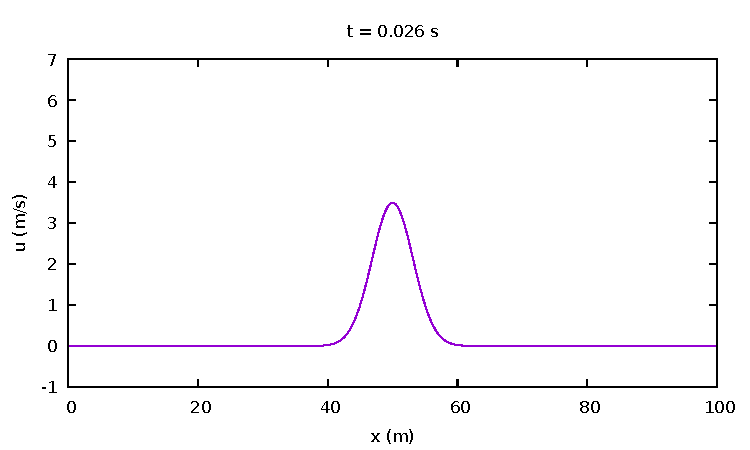
\includegraphics[width=\textwidth]{../burgers1DDF/results/frame001.pdf}
			\caption*{Gráfica de $u(x,t=0.026\unit{\second})$}
			\label{fig:b1ddf1}
		\end{subfigure}\hfill
		\begin{subfigure}{0.4\textwidth}
			\centering
			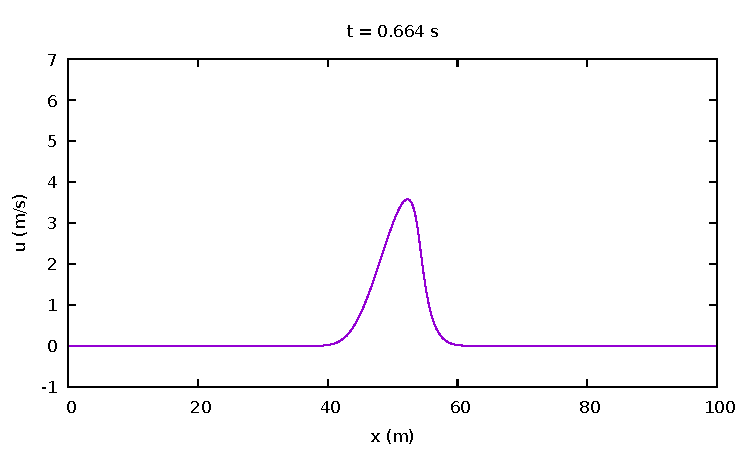
\includegraphics[width=\textwidth]{../burgers1DDF/results/frame026.pdf}
			\caption*{Gráfica de $u(x,t=0.664\unit{\second})$}
			\label{fig:b1ddf2}
		\end{subfigure}\par
		\begin{subfigure}{0.4\textwidth}
			\centering
			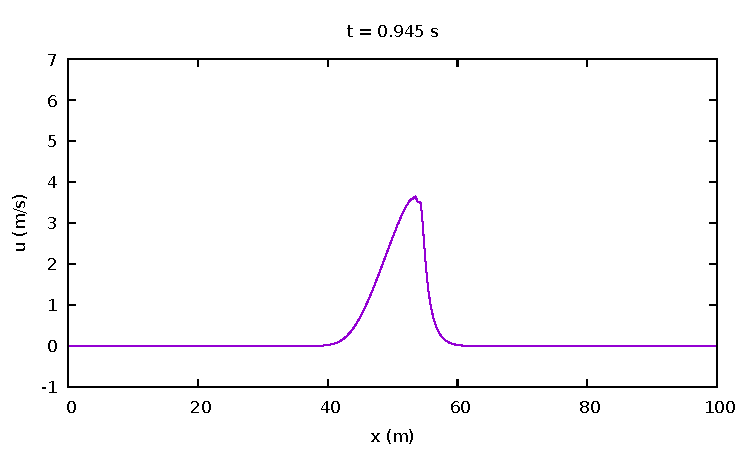
\includegraphics[width=\textwidth]{../burgers1DDF/results/frame037.pdf}
			\caption*{Gráfica de $u(x,t=0.945\unit{\second})$}
			\label{fig:b1ddf3}
		\end{subfigure}\hfill
		\begin{subfigure}{0.4\textwidth}
			\centering
			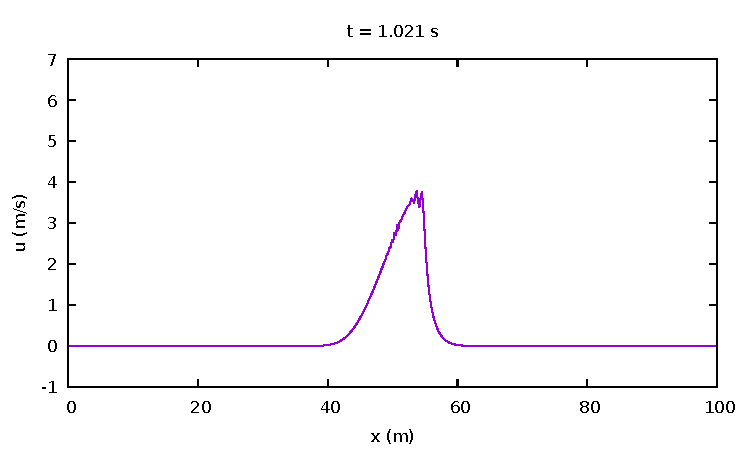
\includegraphics[width=\textwidth]{../burgers1DDF/results/frame040.pdf}
			\caption*{Gráfica de $u(x,t=1.021\unit{\second})$}
			\label{fig:b1ddf4}
		\end{subfigure}\par
		\begin{subfigure}{0.4\textwidth}
			\centering
			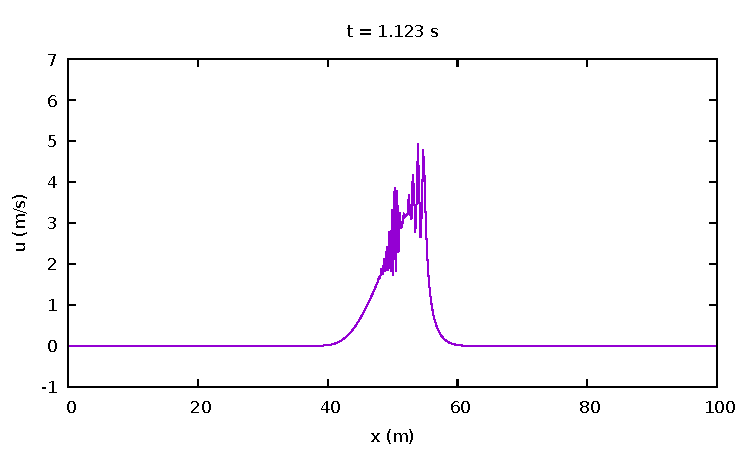
\includegraphics[width=\textwidth]{../burgers1DDF/results/frame044.pdf}
			\caption*{Gráfica de $u(x,t=1.123\unit{\second})$}
			\label{fig:b1ddf5}
		\end{subfigure}\hfill
		\begin{subfigure}{0.4\textwidth}
			\centering
			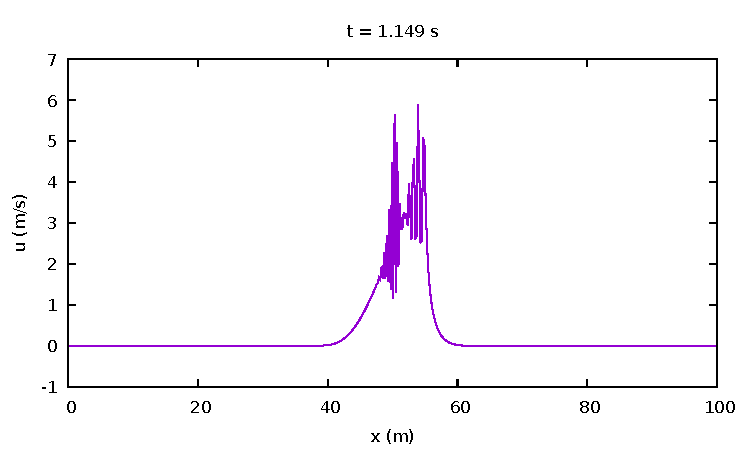
\includegraphics[width=\textwidth]{../burgers1DDF/results/frame045.pdf}
			\caption*{Gráfica de $u(x,t=1.149\unit{\second})$}
			\label{fig:b1ddf6}
		\end{subfigure}
		\caption{Seis instantes de tiempo de la evolución temporal de la ecuación de Burgers no viscosa con diferencias finitas.}
		\label{fig:instantesB1DDF}
	\end{figure}
	
	
	\subsubsection{Discusión de resultados}
	\label{sec:discusion}
	La ecuación de Burgers resuelta con el método de diferencias finitas mostró algunas irregularidades, principalmente la pérdida de continuidad en varias partes de la solución a partir del segundo $1.021$ de la simulación. Este fenómeno es causado gracias al efecto de \textbf{onda de choque}  (o \textbf{shockwave} en inglés) que la ecuación de Burgers presenta. Una onda de choque se define como una discontinuidad en la velocidad de propagación de una onda y dado que la ecuación de Burgers representa la velocidad del fluido modelado, la discontinuidad se manifiesta en la función solución de la ecuación.
	
	Para explicar el fenómeno de onda de choque que se produce en la ec. de Burgers se puede utilizar el \textbf{método de características} para la resolución de la ecuación misma. El método de características consiste en transformar el dominio de la ecuación tal que, en éste, la ecuación diferencial parcial se pueda escribir como un sistema de ecuaciones diferenciales ordinarias, llamadas \textbf{ecuaciones características}. Las curvas del dominio en donde al valuar la ecuación esta se puede escribir como un sistema de ecuaciones diferenciales ordinarias se llaman \textbf{curvas características.}\\
	Para encontrar las curvas características de la ec. de Burgers se necesitan resolver las ecuaciones características: 
	\begin{equation}
		\dv{x}{t} = u(x,t)
		\label{eq:dxdt}
	\end{equation}
	\begin{equation}
		\dv{u}{t} = \pdv{u}{t} + \dv{x}{t}\pdv{u}{x} = \pdv{u}{t}+u\pdv{u}{x} = 0
		\label{eq:parcialu}
	\end{equation}
	Se puede observar en la ecuación \ref{eq:parcialu} que $u$ es constante en el tiempo a lo largo de cualquier curva característica, por lo que resolviendo la ecuación \ref{eq:dxdt} se obtiene:
	\begin{equation}
		x-x_{0} = ut
	\end{equation}
	\begin{equation}
		x(t) = x_{0} + u_{0}(x_0)t
		\label{eq:caracteristica}
	\end{equation}
	Donde $u_0(x) = u(x,0)$
	
	Se puede notar que las curvas características son rectas en el plano $x-t$ que parten de un punto $(x_{n}, 0)$ y poseen pendiente $u_{0}(x_n)$, donde $x_n$ es un punto que pertenece al dominio espacial. Consecuentemente se puede demostrar que estas curvas se intersectarán en un tiempo finito si $u'_{0}(x) < 0$ para algún $x$. Si se supone que las dos características $x(t) = x_{1}+u_{0}(x_1)t$ y $x(t) = x_{2}+u_{0}(x_2)t$ llegan a intersectarse en un tiempo $t_{int}$.
	\begin{equation}
		x_{1}+u_{0}(x_1)t_{int} = x_{2}+u_{0}(x_2)t_{int}
	\end{equation}
	\begin{equation}
		t_{int} = -\frac{x_2-x_1}{u_{0}(x_2) - u_{0}(x_1)}
	\end{equation}
	\begin{equation}
		t_{int} = -\dfrac{1}{\dfrac{u_{0}(x_2) - u_{0}(x_1)}{x_2-x_1}}
	\end{equation}
	\begin{equation}
		t_{int} = -\dfrac{1}{\dfrac{u_{0}(x_2) - u_{0}(x_1)}{x_2-x_1}}
	\end{equation}
	Por el teorema del valor medio, se puede asumir que para un $x_0$ tal que $x_1 < x_0 < x_2$ existe $u'(x_0)=\dfrac{u_{0}(x_2) - u_{0}(x_1)}{x_2-x_1}$ y entonces, $u'$ sí es negativa en algún punto, por lo tanto, el tiempo $t_{int}$ es positivo y las características se intersectan.
	
	Cuando las características se intersectan la onda viajera se rompe ya que según la ecuación diferencial que la rige esta debería seguir siendo constante en dos puntos distintos y esto produce la discontinuidad. El método numérico de diferencias finitas reacciona erróneamente ante la discontinuidad que se presenta en la solución, puesto que el término $u_{i}-u_{i+1}$ es una cantidad que crece cada vez más en cada iteración y el error numérico ya no se puede despreciar, por lo que la solución pierde el significado físico.
	\\
	La segunda irregularidad presentada por los resultados tiene relación con la forma de la ecuación de Burgers, dado que al investigar sobre la resolución numérica se encontró que la ecuación \ref{eq:burgers1d} no es la adecuada para implementar en métodos numéricos, sino la forma conservativa de la misma:
	\begin{equation}
		\pdv{u}{t} + \frac{1}{2}\pdv{(u^2)}{x} = 0
		\label{eq:conservativa}
	\end{equation}
	Con esta ecuación se puede obtener la ecuación \ref{eq:burgers1d} utilizando la regla de la cadena, al igual que calculando la derivada material de $u$; pero esta transformación es válida solamente si la ecuación es diferenciable en todo el dominio, lo cual no sucede en la ecuación de Burgers por el efecto de onda de choque previamente explicado. Por esta razón, es recomendable usar la versión conservativa (ecuación \ref{eq:conservativa}) para resolver la ecuación de Burgers.
	
	Se utilizó esta versión de la ecuación en una simulación usando la discretización siguiente:
	\begin{equation}
		u_{\text{nueva,}i} = u_{i} + \frac{\Delta t}{2\Delta x}(u_{i}^{2}-u_{i+1}^{2}) 
		\label{eq:burgers-conserv-discreta}
	\end{equation}
	En la figura \ref{fig:instantes-conservativa} se muestran cuatro instantes de la solución usando la versión conservativa de la ecuación de Burgers. Se puede notar que en esta solución la onda se propaga mucho más rápido que la onda de la solución de la ecuación de Burgers tradicional, pero también pierde significado físico a causa de la onda de choque. Por tanto el método de diferencias finitas es muy débil para simular la ecuación de Burgers no viscosa.

	\begin{figure}[ht]
		\centering
		\begin{subfigure}[b]{0.4\textwidth}
			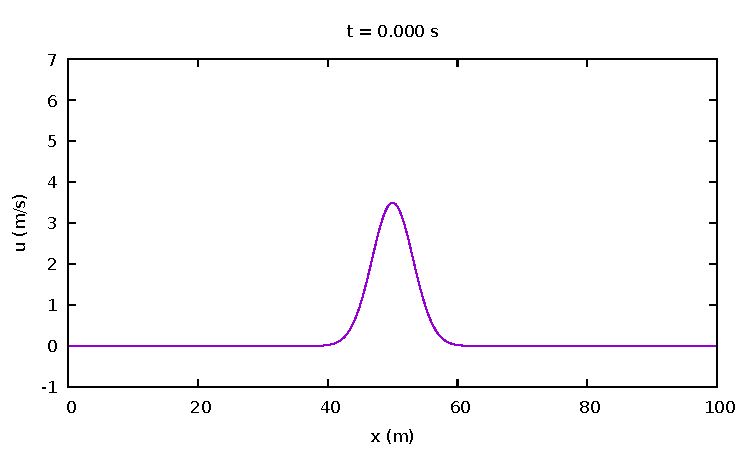
\includegraphics[width=\textwidth]{../burgers1DDF/resultados-conservativa/frame000.pdf}
			\caption*{Gráfica de $u(x,t=0.0\unit{\second})$}
			\label{fig:image1}
		\end{subfigure}
		\hfill
		\begin{subfigure}[b]{0.4\textwidth}
			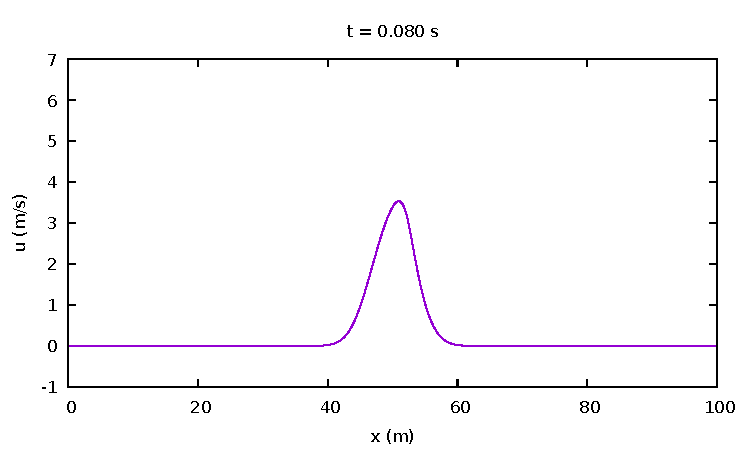
\includegraphics[width=\textwidth]{../burgers1DDF/resultados-conservativa/frame016.pdf}
			\caption*{Gráfica de $u(x,t=0.08\unit{\second})$}
			\label{fig:image2}
		\end{subfigure}
		\par\medskip
		\begin{subfigure}[b]{0.4\textwidth}
			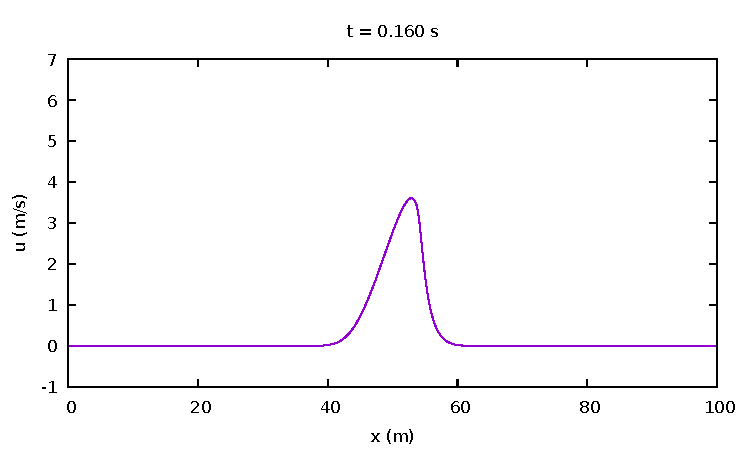
\includegraphics[width=\textwidth]{../burgers1DDF/resultados-conservativa/frame032.pdf}
			\caption*{Gráfica de $u(x,t=0.016\unit{\second})$}
			\label{fig:image3}
		\end{subfigure}
		\hfill
		\begin{subfigure}[b]{0.4\textwidth}
			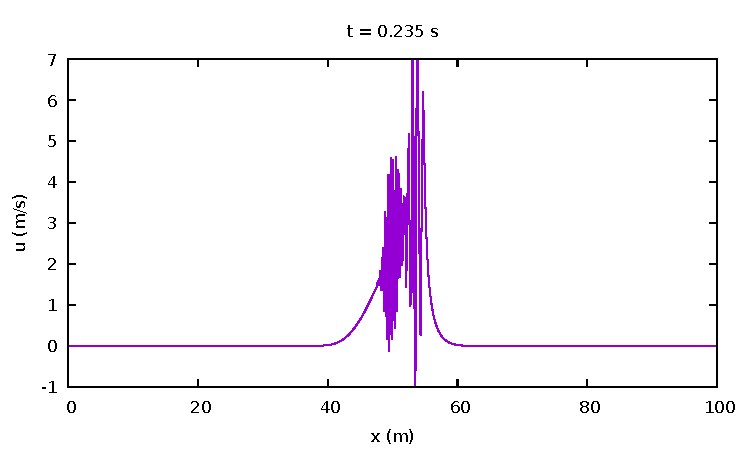
\includegraphics[width=\textwidth]{../burgers1DDF/resultados-conservativa/frame047.pdf}
			\caption*{Gráfica de $u(x,t=0.0235\unit{\second})$}
			\label{fig:image4}
		\end{subfigure}
		\caption{Cuatro instantes de tiempo de la evolución temporal de la ecuación de Burgers en su versión conservativa, con diferencias finitas.}
		\label{fig:instantes-conservativa}
	\end{figure}
	
	\newpage
	\subsection{Ecuación de Burgers viscosa, en una dimensión}
	\label{sec:burg-vis1ddf}
	\subsubsection{Descripción del problema}
	La ecuación de Burgers viscosa es una ecuación diferencial parcial no lineal de \textbf{segundo orden,} que se utiliza para modelar la velocidad de gases o fluidos con viscosidad considerable. La ecuación tiene la siguiente forma:
	\begin{equation}
		\pdv{u}{t}+u\pdv{u}{x}=\nu \pdv{^2 u}{x^2}
		\label{eq:burg-vis}
	\end{equation}
	Donde $\nu$ es el coeficiente de viscosidad del medio modelado. Cabe destacar que $\nu$ es el inverso del \textbf{número de Reynolds} $Re$, una cantidad adimensional que sirve para medir la proporción entre fuerzas inerciales y viscosas. 

	En consecuencia de haber obtenido distintos resultados en la sección \ref{sec:burgers1ddf} al utilizar la versión conservativa (\ref{eq:conservativa}) y no conservativa (\ref{eq:burgers1d}) de la ecuación de Burgers no viscosa, para este problema se optó por resolver la versión conservativa con el término de viscosidad incluido.
	\begin{equation}
		\pdv{u}{t}+\frac{1}{2}\pdv{(u^2)}{x}=\nu \pdv{^2 u}{x^2}
		\label{eq:burg-vis-con}
	\end{equation}
	
 	La ecuación \ref{eq:burg-vis-con} se resolvió en el mismo dominio espacial $I$ y bajo las mismas condiciones iniciales y de frontera que la versión no viscosa de la sección \ref{sec:burgers1ddf}. 
 	\begin{equation}
 		u(0,0)=0
 	\end{equation}
 	\begin{equation}
 		u(\text{L},0)= 0
 	\end{equation}
	\begin{equation}
		u(x,0) = A\exp(-b(x-\mu)^{2})
		\label{eq:condinicial-vis}
	\end{equation}
	\\
	Donde:
	\begin{itemize}
		\item $L = 100\unit{\meter}$
		\item $A=3.5\mpers$
		\item $b=0.05$
		\item $\mu=L/2=50\unit{\meter}$
	\end{itemize}
	
	Se resolvieron tres ecuaciones con un coeficiente de viscosidad $\nu$ distinto para cada una:$0.50\unit{m^{2}\per s}$, $1.60\unit{m^{2}\per s}$ y $3.0\unit{m^{2}\per s}$.
	\subsubsection{Aplicación del método y código implementado}
	Para este problema se utilizó como código base el programa de la solución no viscosa, haciendo algunos cambios; por ejemplo, el del tiempo de simulación total y la impresión de datos.
	\lstinputlisting[title = Variables generales de la simulación,
	language = C++,
	firstline=24,
	lastline=64,
	keywordstyle=\color{blue}]{../burg-vis1DDF/burg-vis1DDF.cpp}
	Como puede notarse en el código presentado, los archivos \texttt{.dat} y \texttt{.gp} están nombrados de acuerdo al coeficiente de viscosidad utilizado en la solución que representan.
	
	Se aplicó la discretización de la ecuación \ref{eq:segunda-derivada-discreta} para tratar la derivada de segundo orden de la ecuación de Burgers viscosa. Aplicando las discretizaciones en la ecuación \ref{eq:burg-vis-con} se obtiene:
	
	\begin{equation}
		\frac{u_{\text{nueva},i}-u_{i}}{\Delta t} +  \frac{1}{2} \left(\frac{u^{2}_{i+1}-u^{2}_{i}}{\Delta x}\right)  -  \nu \left( \frac{u_{i+1}-2u_{i}+u_{i-1}}{(\Delta x)^{2}} \right) =0
	\end{equation}
	\begin{equation}
		u_{\text{nueva},i} = u_{i} + \frac{\Delta t}{2 \Delta x} \left( u^{2}_{i}-u^{2}_{i+1} \right)  + \nu \frac{\Delta t}{(\Delta x)^2}\left( u_{i+1}-2u_{i}+u_{i-1} \right) 
	\end{equation}
	A continuación se muestra el ciclo principal de integración numérica de la ecuación de Burgers viscosa
	
	\lstinputlisting[title = Ciclo principal de integración,
	language = C++,
	firstline = 91,
	lastline = 114,
	keywordstyle = \color{blue}]{../burg-vis1DDF/burg-vis1DDF.cpp}
	
	\subsubsection{Resultados}
	Se graficaron las tres soluciones obtenidas con los diferentes coeficientes de viscosidad considerados \footnote{En la viñeta de cada gráfica, $\nu$ esta escrito como \textbf{nu}}. Se muestran en la figura \ref{fig:instantesvis1DDF} las gráficas para seis instantes de tiempo en orden ascendente. La animación completa de la simulación está disponible en el siguiente \href{https://github.com/highchen147/practicas/blob/main/burg-vis1DDF/results/simulacion.mp4}{enlace.}
	
	\begin{figure}[ht]
		\centering
		\begin{subfigure}{0.4\textwidth}
			\centering
			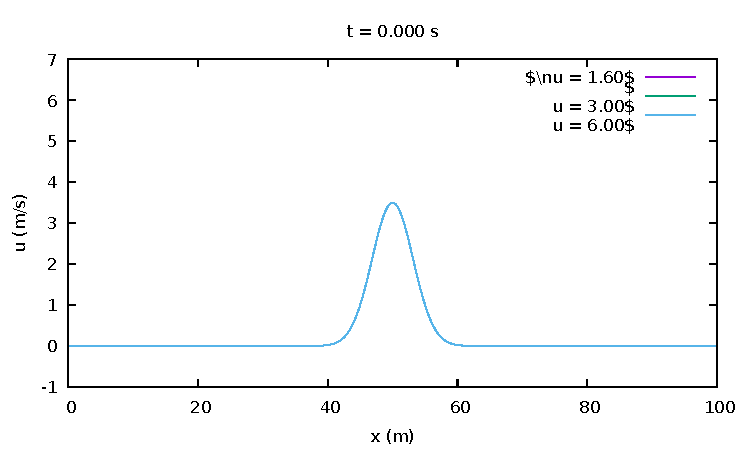
\includegraphics[width=\textwidth]{../burg-vis1DDF/results/frame000.pdf}
			\caption*{Gráficas para $t=0.00\unit{\second}$}
			\label{fig:vis1ddf1}
		\end{subfigure}\hfill
		\begin{subfigure}{0.4\textwidth}
			\centering
			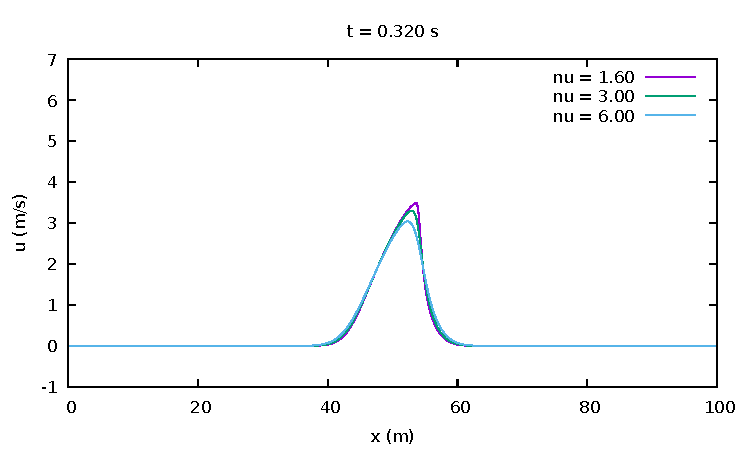
\includegraphics[width=\textwidth]{../burg-vis1DDF/results/frame016.pdf}
			\caption*{Gráficas para $t=0.032\unit{\second}$}
			\label{fig:vis1ddf2}
		\end{subfigure}\par
		\begin{subfigure}{0.4\textwidth}
			\centering
			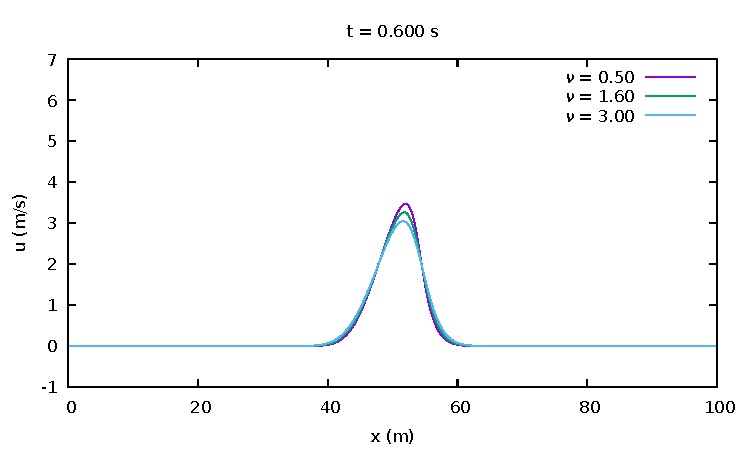
\includegraphics[width=\textwidth]{../burg-vis1DDF/results/frame030.pdf}
			\caption*{Gráfica de $u(x,t=0.32\unit{\second})$}
			\label{fig:vis1ddf3}
		\end{subfigure}\hfill
		\begin{subfigure}{0.4\textwidth}
			\centering
			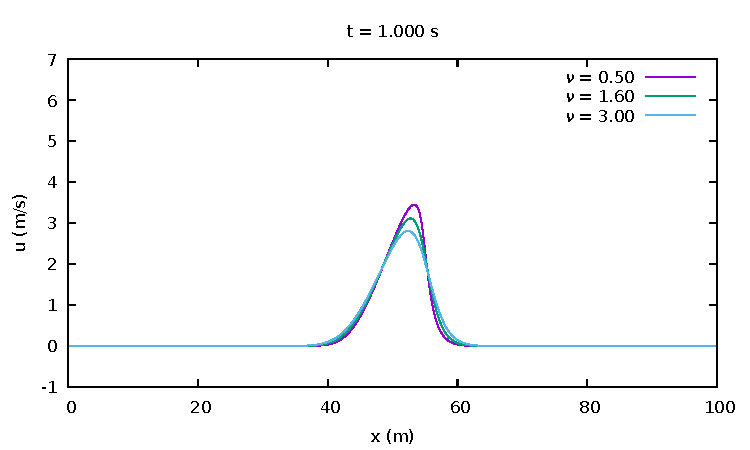
\includegraphics[width=\textwidth]{../burg-vis1DDF/results/frame050.pdf}
			\caption*{Gráfica de $u(x,t=1.0\unit{\second})$}
			\label{fig:vis1ddf4}
		\end{subfigure}\par
		\begin{subfigure}{0.4\textwidth}
			\centering
			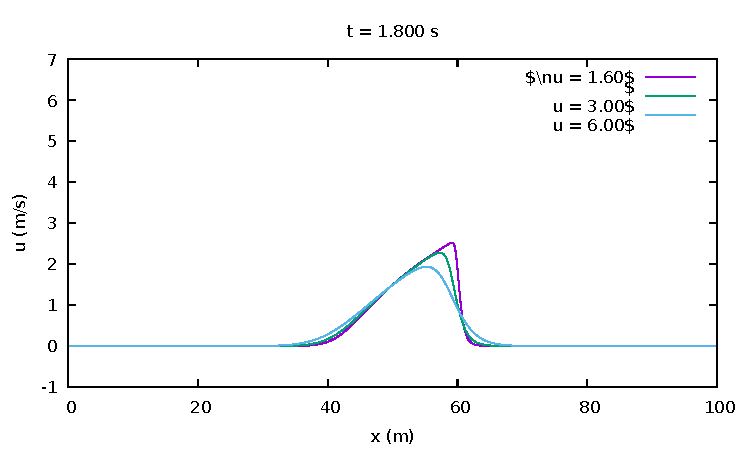
\includegraphics[width=\textwidth]{../burg-vis1DDF/results/frame090.pdf}
			\caption*{Gráfica de $u(x,t=1.8\unit{\second})$}
			\label{fig:vis1ddf5}
		\end{subfigure}\hfill
		\begin{subfigure}{0.4\textwidth}
			\centering
			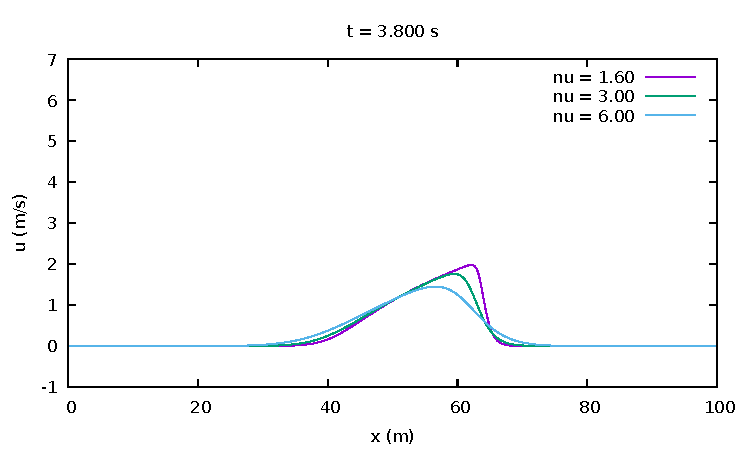
\includegraphics[width=\textwidth]{../burg-vis1DDF/results/frame190.pdf}
			\caption*{Gráfica de $u(x,t=3.8\unit{\second})$}
			\label{fig:vis1ddf6}
		\end{subfigure}
		\caption{Seis instantes de tiempo de la evolución temporal de tres versiones de la ecuación de Burgers viscosa para diferentes coeficientes de viscosidad, con diferencias finitas.}
		\label{fig:instantesvis1DDF}
	\end{figure}
	\subsubsection{Discusión de resultados}
	La solución numérica de la ecuación de Burgers viscosa proporciona una comprensión más coherente de la evolución temporal de la velocidad de un fluido modelado en comparación con la ecuación de Burgers no viscosa. Esto se debe a que la solución numérica no presenta irregularidades considerables o efectos que hagan perder el significado físico del sistema. Según lo investigado, los métodos más frecuentemente utilizados para resolver la ecuación de Burgers suelen incluir un término viscoso para calibrar y afinar la solución que se desea analizar. Esto es lógico, ya que en la dinámica de un gas o fluido real siempre estará presente algún nivel de viscosidad.
	
	Al resolver este problema se consideraron varios valores para el coeficiente de viscosidad $\nu$, como se puede ver en la figura \ref{fig:instantesvis1DDF}. Cabe destacar que $\nu = 0.5$ fue el valor mínimo que este pudo tener sin que la solución perdiera significado físico. Por lo tanto, el método de diferencias finitas está limitado a resolver la ecuación viscosa de Burgers con $\nu > 0.5$; no obstante, el método es mucho más útil al resolver la versión viscosa que la versión no viscosa de la ecuación de Burgers, ya que hay soluciones que no presentan error numérico considerable. En la figura \ref{fig:instantes-nu0.3} se pueden observar cuatro instantes de tiempo de la solución de la ecuación viscosa con $\nu = 0.3$ utilizando diferencias finitas.
	
	\begin{figure}[ht]
		\centering
		\begin{subfigure}[b]{0.4\textwidth}
			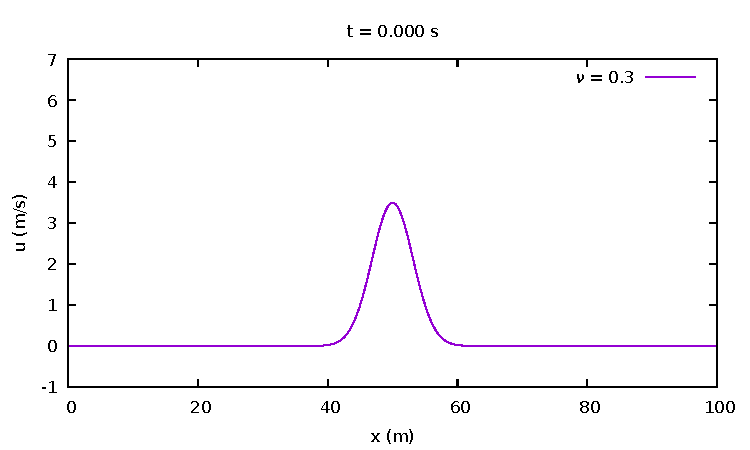
\includegraphics[width=\textwidth]{../burg-vis1DDF/results/frames0.3/frame000.pdf}
			\caption*{Gráfica de $u(x,t=0.0\unit{\second})$}
			\label{fig:vis0.3-1}
		\end{subfigure}
		\hfill
		\begin{subfigure}[b]{0.4\textwidth}
			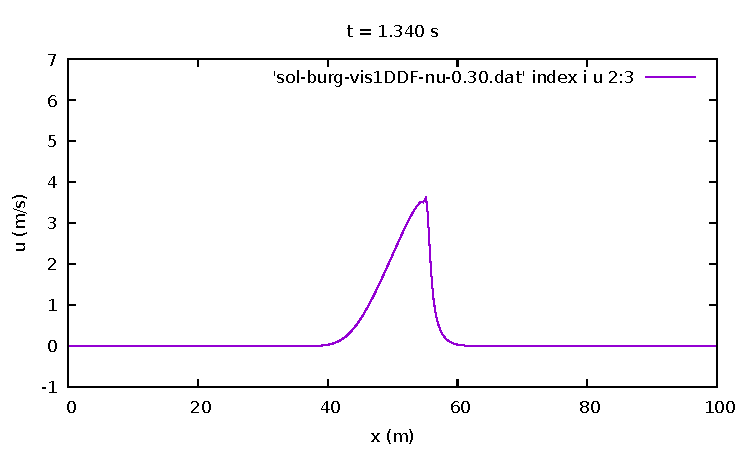
\includegraphics[width=\textwidth]{../burg-vis1DDF/results/frames0.3/frame067.pdf}
			\caption*{Gráfica de $u(x,t=1.34\unit{\second})$}
			\label{fig:vis0.3-2}
		\end{subfigure}
		\par\medskip
		\begin{subfigure}[b]{0.4\textwidth}
			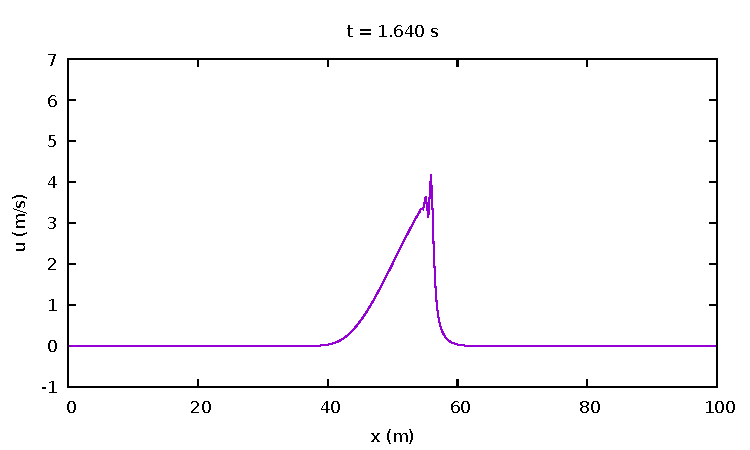
\includegraphics[width=\textwidth]{../burg-vis1DDF/results/frames0.3/frame082.pdf}
			\caption*{Gráfica de $u(x,t=1.64\unit{\second})$}
			\label{fig:vis0.3-3}
		\end{subfigure}
		\hfill
		\begin{subfigure}[b]{0.4\textwidth}
			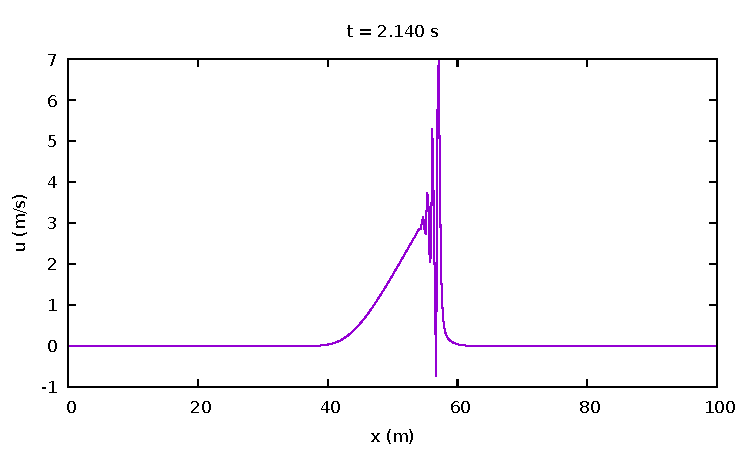
\includegraphics[width=\textwidth]{../burg-vis1DDF/results/frames0.3/frame107.pdf}
			\caption*{Gráfica de $u(x,t=2.14\unit{\second})$}
			\label{fig:vis0.3-4}
		\end{subfigure}
		\caption{Cuatro instantes de tiempo de la evolución temporal de la ecuación de Burgers con viscosidad igual a $0.3$, resuelta con diferencias finitas.}
		\label{fig:instantes-nu0.3}
	\end{figure}

	\theoremstyle{definition}
	\newtheorem{definition}{Definición}[section]
	\section{Método de volúmenes finitos}
	El siguiente método utilizado fue el \textbf{método de volúmenes finitos.} Este método se especializa en resolver ecuaciones diferenciales escritas en forma conservativa y es capaz de integrarlas aún cuando las soluciones poseen discontinuidades o  en el contexto de las ecuaciones de la mecánica de fluidos, choques (\textit{shocks} en inglés) \cite{LeVeque1998}. El método de volúmenes finitos es aplicable utilizando métodos llamados \textit{esquemas} o \textit{marcos}, que sirven para calcular apropiadamente el \textbf{flujo} en las interfaces de las celdas de la grilla \cite{LeVeque1998}. Se explicará la deducción del método de volúmenes finitos, los marcos utilizados y la teoría de su funcionamiento.
	
	El principio básico del método de volúmenes finitos es la reinterpretación de los valores discretizados $u_{i}^{n}$ de la función incógnita $u$; dado que en lugar de considerar a estos valores como la aproximación del valor exacto $u(x_{i}, t_{n}) $\footnote{La notación introducida $u_{i}^{n}$ $\approx$ $u(x_{i}, t_{n})$ es tal que, $t_n \equiv n \Delta t $ con $n \in \mathbb{N}$} se interpretan como el \textbf{valor promedio} de la función $u$ en el intervalo $C_{i} = \left[ x_i, x_{i+1} \right]$, también denominado \textbf{celda}. Entonces la discretización de la función consiste en dividir el intervalo $I = [0,L]$ en $N$ intervalos $C_i$, donde $\Delta x = L/N = x_{i+1} - x_i$. De tal manera que, formalmente, el valor $u_{i}^{n}$ se calcula con una integral en $x$ sobre $C_i$:
	
	\begin{equation}
		u_{i}^{n} \approx \frac{1}{\Delta x} \int_{C_i} u(x,t_n) \dd{x} \equiv \frac{1}{\Delta x} \int_{x_i}^{x_{i+1}} u(x,t_n) \dd{x}
		\label{eq:uiapprox}
	\end{equation}
	
	Ahora, el método toma ventaja de esta nueva interpretación de la discretización cuando se integra la versión conservativa de la ecuación diferencial a resolver, es decir, una ecuación de la forma:
	\begin{equation}
		\pdv{u}{t} + \pdv{f(u)}{x} = 0
		\label{eq:conservative_general}
	\end{equation}
	
	donde $f(u)$ es la función del flujo de $u$; para la ecuación de Burgers $f(u) = \frac{u^2}{2}$. Entonces, integrando dicha ecuación en ambas variables:
	
	\begin{equation}
		\int_{C_i} \pdv{u}{t} \dd{x} + \int_{C_i} \pdv{f(u)}{x} \dd{x} = 0
		\label{eq:ecuacion-integrada}
	\end{equation}

	\begin{equation}
		\int_{C_i} \pdv{u}{t} \dd{x} + f(u(x_{i+1} ,t)) - f(u(x_{i},t)) = 0
	\end{equation}

	\begin{equation}
		\int_{t_n}^{t_{n+1}} \int_{C_i} \pdv{u}{t} \dd{x} \dd{t} + \int_{t_n}^{t_{n+1}}\left[ f(u(x_{i+1} ,t)) - f(u(x_{i},t))\right]\dd{t} = 0
	\end{equation}

	\begin{equation}
		\int_{C_i} \left[u(x, t_{n+1}) - u(x, t_n)\right] \dd{x} + \int_{t_n}^{t_{n+1}}\left[ f(u(x_{i+1} ,t)) - f(u(x_{i},t))\right]\dd{t} = 0 
	\end{equation}
	
	Esta última expresión es totalmente exacta y expresa cómo cambiará el valor promedio de $u$ en cada celda, después de un instante $\Delta t$. Ahora, haciendo uso de la aproximación de la ecuación \ref{eq:uiapprox}, se tiene:
	\begin{equation}
		 \Delta x\left( u_{i}^{n+1} - u_{i}^{n}\right)   + \int_{t_n}^{t_{n+1}}\left[ f(u(x_{i+1} ,t)) - f(u(x_{i},t))\right]\dd{t} = 0 
	\end{equation}

	\begin{equation}
		u_{i}^{n+1} - u_{i}^{n} + \frac{1}{\Delta x}\int_{t_n}^{t_{n+1}}\left[ f(u(x_{i+1} ,t)) - f(u(x_{i},t))\right]\dd{t} = 0 
	\end{equation}

	Por otro lado, la siguiente integral se puede interpretar como el flujo promedio en el intervalo temporal $[t_n,t_{n+1}]$. Esto es:
	\begin{equation}
		F_{i}^{n} \approx \frac{1}{\Delta t} \int_{t_n}^{t_{n+1}} f(u(x_i,t)) \dd{t}
		\label{eq:flujo_promedio}
	\end{equation}
	Sustituyendo en la integración de la ecuación, se obtiene:
	\begin{equation}
		u_{i}^{n+1} - u_{i}^{n} + \frac{\Delta t}{\Delta x}\left[ F_{i+1}^n - F_{i}^{n}\right] = 0
		\label{eq:diferencia-flujos}
	\end{equation}
	Entonces, la ecuación \ref{eq:diferencia-flujos} es la forma de \textbf{diferencia de flujos} de la ecuación de conservación; y a partir de la misma se pueden desarrollar los métodos numéricos basados en el método de volúmenes finitos, puesto que la función $F_{i}^{n}$ es una aproximación numérica. Para que el método funcione, la función $F_{i}^{n}$ debe calcularse utilizando los valores de la grilla, $u^{n}$ de tal manera que se obtenga un método numérico totalmente discretizado \cite{LeVeque1998}. 
	
	Se dice que la ecuación \ref{eq:diferencia-flujos} es un método numérico \textbf{conservativo} ya que emula la idea de la solución exacta expuesta en el desarrollo del inicio de este capítulo (ecuación \ref{eq:ecuacion-integrada}). Si se suman los valores que toma $u$, desde la celda $L$ hasta la celda $R$, se obtiene:
	\begin{equation}
		\sum_{i=L}^{R} u_{i}^{n+1} - \sum_{i=L}^{R}  u_{i}^{n} + \frac{\Delta t}{\Delta x}\left[ \sum_{i=L}^{R}F_{i+1}^{n} - \sum_{i=L}^{R}F_{i}^{n}\right] =0
	\end{equation}
		
	\begin{equation}
		{\Delta x}\sum_{i=L}^{R} u_{i}^{n+1} - {\Delta x}\sum_{i=L}^{R}  u_{i}^{n} + {\Delta t}\left[ F_{R+1}^{n} - F_{L}^{n} \right] =0
	\end{equation}
	Entonces, se concluye que el resultado del equivalente discreto de la integración de la función $u$ varía en el tiempo solamente debido a los flujos en las celdas limitantes del dominio considerado. Esta es la propiedad conservativa de la ecuación de diferencia de flujos.
	
	Volviendo a considerar el flujo $F_{i}^{n}$, se puede notar en la ecuación \ref{eq:flujo_promedio} que la expresión para el flujo promedio en una interfaz, $F_{i}^{n}$ contiene una integral y generalmente, en consecuencia de que $u$ depende del tiempo, esta integral no es trivial. Sin embargo, se sabe que la información de la onda se propaga a través del espacio con una velocidad finita, lo que implica que es posible obtener $F_{i}^{n}$ a partir de los valores $u_i$ y $u_{i-1}$ \cite{LeVeque1998}:
	\begin{equation}
		F_{i}^{n} = F(u_{i-1}^{n}, u_{i}^{n})
	\end{equation}
	De tal manera que, sustituyendo en la ecuación \ref{eq:diferencia-flujos} se obtiene:
	\begin{equation}
		u_{i}^{n+1} - u_{i}^{n} + \frac{\Delta t}{\Delta x}\left[ F(u_{i}^{n}, u_{i+1}^{n}) - F(u_{i-1}^{n}, u_{i}^{n})\right] = 0
		\label{eq:flux-diff}
	\end{equation}
	A continuación se explican los marcos numéricos evaluados para calcular el flujo numérico $F_{i}^{n}$ para resolver la ecuación de Burgers, donde $f(u)=\frac{u^2}{2}$.
	
	\subsection{Esquema de Lax-Friedrichs}
	La primera expresión que lógicamente se puede proponer para poder calcular $F(u_{i-1}^{n}, u_{i}^{n})$ es promediar el valor del flujo $f(u)$ valuado en $u_{i-1}^{n}$ y en $u_{i}^{n}$; esto es:
	\begin{equation}
		F(u_{i-1}^{n}, u_{i}^{n}) = \frac{1}{2} \left( f(u_{i-1}^{n}) + f(u_{i}^{n})\right) 
	\end{equation}
	\begin{equation}
		F(u_{i-1}^{n}, u_{i}^{n}) = \frac{1}{2} \left( (u_{i-1}^{n})^2 + (u_{i}^{n})^2 \right) 
	\end{equation}
	
	Sin embargo, esta elección para el flujo numérico no proporciona una integración estable para ningún valor de $\frac{\Delta t}{\Delta x}$ \cite{LeVeque1998}. Por tanto, se le agrega un término al flujo que actúa como un \textit{flujo difusivo} y compensa parcialmente los efectos de las discontinuidades en las soluciones. En el método de Roe se explicará la razón de la inclusión de este término.
	\begin{equation}
		{\boxed{F(u_{i-1}^{n}, u_{i}^{n}) = \frac{1}{2} \left( (u_{i-1}^{n})^2 + (u_{i}^{n})^2 \right)  - \frac{\Delta t}{2\Delta x}(u_{i}^{n}-u_{i-1}^{n})} }
	\end{equation}
	Este es el esquema de Lax-Friedrichs para el flujo numérico de la ecuación de Burgers.
	
	\subsection{Esquema de Godunov}
	El esquema de Godunov se justifica a través de conceptos avanzados de las ecuaciones diferenciales de conservación; pero la idea fundamental del método es simple. El esquema de Godunov consiste en resolver el \textbf{problema de Riemann} en cada una de las celdas de la solución, este problema se explicará con detalle después de considerar algunas propiedades de las ecuaciones diferenciales en forma conservativa. Primero, se debe comprender el concepto de \textbf{solución débil} de una ecuación diferencial.
	\subsubsection{Solución débil de una ecuación diferencial}
	Como fue visto en secciones anteriores, la ecuación de Burgers tiene soluciones discontinuas, lo cual parece contradecir la misma ecuación diferencial puesto que esta posee derivadas parciales en todas sus variables y una función discontinua no es derivable en todo su dominio. Con el objetivo de validar las funciones discontinuas como soluciones de las ecuaciones diferenciales el concepto de solución débil fue introducido a la teoría de ecuaciones diferenciales parciales \cite{Cameron}.
	
	Como motivación para hacer riguroso el concepto de la solución débil se define una función infinitamente suave $\phi(x,t)$ que posee un soporte compacto, es decir, que la función es distinta de cero solamente en un subconjunto compacto del espacio $(x,t)= \mathbb{R} \times \left[ 0, + \infty \right] $. Luego se define $u(x,t)$ tal que esta satisface la ecuación de conservación general $\pdv{u}{t} + \pdv{f(u)}{x}=0$. Entonces integrando por partes se obtiene lo siguiente:
	\begin{equation}
		\int_{0}^{\infty}\int_{-\infty}^{\infty}\left( \pdv{u}{t} + \pdv{f(u)}{x} \right)\phi(x,t)\dd{x}\dd{t} = 0
		\label{eq:integral_conservative1}
	\end{equation}
	 
	 \begin{equation}
	 	\left( \int_{-\infty}^{\infty} \phi u \dd{x} \right)\bigg|_{0}^{\infty} - \int_{0}^{\infty}\int_{-\infty}^{\infty}\left( u\pdv{\phi}{t} + f(u)\pdv{\phi}{x}\right)\dd{x}\dd{t}=0
	 	\label{eq:integral_conservative2}
	 \end{equation}
	A partir de este resultado, yace la definición de solución débil.
	
	
	
	\begin{definition}
		$u(x,t)$ es una solución débil de la ecuación diferencial $\pdv{u}{t} + \pdv{f(u)}{x}=0$ si para cualquier función suave $\phi(x,t)$ con soporte compacto se satisface lo siguiente:
		\begin{equation}
			\int_{0}^{\infty}\int_{-\infty}^{\infty}\left( u\pdv{\phi}{t} + f(u)\pdv{\phi}{x}\right)\dd{x}\dd{t}=\left( \int_{-\infty}^{\infty} \phi u \dd{x} \right)\bigg|_{0}^{\infty}=-\int_{-\infty}^{\infty}\phi (x,0)u(x,0)\dd{x}
			\label{eq:weak_sol_cond}
		\end{equation}
	\end{definition}
	Se puede notar que la definición de la solución débil fuerza que la función $u(x,t)$ satisfaga la forma integral de la ecuación conservativa (\ref{eq:integral_conservative1}), mediante la función $\phi$ denominada \textit{función de prueba} \cite{Cameron}.
	
	\subsubsection{Problema de Riemann}
	El problema de Riemann es un problema de valores iniciales para cualquier ecuación diferencial en forma conservativa (ecuación \ref{eq:conservative_general}), que exige:
	\begin{equation}
		u(x,0) =
		\begin{cases}
			u_{L} & x < 0 \\
			u_{R} & x > 0
		\end{cases}
	\end{equation}
	Se considerarán los casos no triviales para este problema, si $u_L > u_R$ o $u_L < u_R$.
	\subsubsection{Caso $u_L > u_R$ del problema de Riemann}
	Este caso (apreciable en la figura \ref{fig:riemann_caso1}) de condición inicial tiene como solución general de una ecuación de conservación (ecuación \ref{eq:conservative_general}):
	\begin{equation}
		u(x,t) =
		\begin{cases}
			u_{L} & x < st \\
			u_{R} & x > st
		\end{cases}
		\qquad \text{donde,}
		\qquad
		\begin{aligned}
			s &= \frac{f(u_L) - f(u_R)}{u_L - u_R}
		\end{aligned}
		\label{eq:sol-riemann-weak}
	\end{equation}
	Donde $s$ es la \textit{velocidad de choque.} La expresión para $s$ también es denominada \textit{condición Rankine-Hugoniot} \cite{Cameron}. A continuación se demostrará que esta solución es una solución débil de la ecuación (\ref{eq:conservative_general}).\\
		
	\begin{figure}[h]
		\centering
		\begin{tikzpicture}[scale=1.5]
			\draw[stealth-stealth] (-2,0) -- (2,0) node[right] {$x$};
			\draw[-] (0,-1.5) -- (0,1.5) node[above] {$u(x,0)$};
			\draw[domain=-2:0,smooth,variable=\x,blue] plot ({\x},{1});
			\draw[domain=0:2,smooth,variable=\x,red] plot ({\x},{-1});
			\draw[dashed] (0,-1.5) -- (0,1.5);
		\end{tikzpicture}
		\caption{Gráfica de condición inicial del caso $u_L > u_R$}
		\label{fig:riemann_caso1}
	\end{figure}
	\textit{Prueba:} Sea $\phi$ una función de prueba con soporte compacto $U$ y que este último yace completamente en alguno de los dos conjuntos siguientes: $\{x<st\}$ o $\{x>st\}$. Dado que $u(x,t)$ es constante en ambos conjuntos mencionados, esta satisface la ecuación conservativa (\ref{eq:integral_conservative1}) y consecuentemente se satisface la condición \ref{eq:weak_sol_cond}\cite{Cameron}.
	
	Ahora se demostrará que $u(x,t)$ es la única solución débil de la ecuación \ref{eq:conservative_general}. Suponiendo que el soporte $U$ de $\phi$ está dividido por la recta $x=st$, de tal forma que el conjunto a la izquierda de la recta es $U_L$ y a la derecha es $U_R$. Integrando, se obtiene 
	\begin{equation}
		\int_{0}^{\infty}\int_{-\infty}^{\infty}\left( u\pdv{\phi}{t} + f(u)\pdv{\phi}{x}\right)\dd{x}\dd{t} = \int\int_{U_L}\left( u\pdv{\phi}{t} + f(u)\pdv{\phi}{x}\right)\dd{x}\dd{t} + \int\int_{U_R}\left( u\pdv{\phi}{t} + f(u)\pdv{\phi}{x}\right)\dd{x}\dd{t}
		\label{eq:integracion-cons}
	\end{equation}
	
	Usando el teorema de Green
	\begin{equation}
		\int\int_{D} \left(\pdv{P}{x} -\pdv{Q}{t}\right)\dd{x}\dd{t} = \int\int_{\partial D} P\dd{t} + Q\dd{x}
	\end{equation}
	y dado que $u(x,t)$ es constante tanto en $U_L$ como en $U_R$ se tiene que:
	\begin{equation}
		\pdv{(u\phi)}{t} = u\pdv{\phi}{t} 
	\end{equation}
	\begin{equation}
		\pdv{(f(u)\phi)}{x} = f(u)\pdv{\phi}{x} 
	\end{equation}	
	Aplicando estas propiedades en la integración \ref{eq:integracion-cons}, se obtiene
	\begin{equation}
		\int_{0}^{\infty}\int_{-\infty}^{\infty}\left( u\pdv{\phi}{t} + f(u)\pdv{\phi}{x}\right)\dd{x}\dd{t} = \int\int_{U_L}\left( \pdv{(u\phi)}{t} + \pdv{(f(u)\phi)}{x}\right)\dd{x}\dd{t} + \int\int_{U_R}\left( \pdv{(u\phi)}{t} + \pdv{(f(u)\phi)}{x}\right)\dd{x}\dd{t}
	\end{equation}

	\begin{equation}
		\int_{0}^{\infty}\int_{-\infty}^{\infty}\left( u\pdv{\phi}{t} + f(u)\pdv{\phi}{x}\right)\dd{x}\dd{t}=\int_{\partial U_L}\phi \left( f(u_L)\dd{t} - u_L \dd{x}\right) + \int_{\partial U_R}\phi \left( f(u_R)\dd{t} - u_R \dd{x}\right)
	\end{equation}
	\begin{equation}
		\int_{0}^{\infty}\int_{-\infty}^{\infty}\left( u\pdv{\phi}{t} + f(u)\pdv{\phi}{x}\right)\dd{x}\dd{t}=\int_{x=st}\phi \left(\frac{f(u_L)}{s} - u_L  - \frac{f(u_R)}{s} + u_R  \right)\dd{x}-\int_{-\infty}^{0}\phi u_L \dd{x} -\int_{0}^{\infty}\phi u_R \dd{x}
	\end{equation}
	\begin{equation}
		\int_{0}^{\infty}\int_{-\infty}^{\infty}\left( u\pdv{\phi}{t} + f(u)\pdv{\phi}{x}\right)\dd{x}\dd{t}=\int_{x=st}\phi \left(\frac{f(u_L)-f(u_R)}{s} - (u_L-u_R) \right)\dd{x} - \int_{-\infty}^{\infty}\phi(x,0)u(x,0) \dd{x}
		\label{eq:integracion-final}
	\end{equation}
	El integrando del primer término de la ecuación (\ref{eq:integracion-final}) se hace cero si y solo si $s = \frac{f(u_L) - f(u_R)}{u_L - u_R}$ y dado que esta integral debe ser cero por la condición \ref{eq:weak_sol_cond}, se demuestra que $u(x,t)$ definida en \ref{eq:sol-riemann-weak} es la única solución para el problema de Riemann en el caso $u_L > u_R$.
	
	Si se sustituye el flujo de la ecuación de Burgers, se encuentra que la solución del problema de Riemann de esta ecuación, para este caso es 
	
	\begin{equation}
		u(x,t) =
		\begin{cases}
			u_{L} & x < st \\
			u_{R} & x > st
		\end{cases}
		\qquad \text{donde,}
		\qquad
		\begin{aligned}
			s &= \frac{u_{L} + u_{R}}{2}
		\end{aligned}
		\label{eq:sol-riemann-weak-burgers}
	\end{equation}

	\subsubsection{Caso $u_L < u_R$ del problema de Riemann}
	
	Hay múltiples soluciones débiles para este caso. Por  ejemplo, se puede demostrar que la solución \ref{eq:sol-riemann-weak-burgers} satisface este caso también, tomando en cuenta que cambiará el signo de la velocidad de propagación $s$. Sin embargo esta solución no satisface la condición de entropía descrita por \cite{Cameron}.
	
	\begin{definition}
		Una discontinuidad, propagándose en el espacio $x-t$, dada por la ecuación \ref{eq:sol-riemann-weak}, satisface la condición de entropía si $f'(u_l)>s>f'(u_R)$.
	\end{definition}
	 Para la ecuación de Burgers, esta última condición equivale a $u_L > u_R$. Entonces la solución físicamente válida, o que satisface la condición de entropía, se encuentra resolviendo analíticamente el problema de Riemann para la ecuación de Burgers con viscosidad (ecuación \ref{eq:burg-vis}) y luego en la solución, hacer tender a cero el parámetro de viscosidad $\nu$. Según \cite{Cameron}, la solución débil que se obtiene es
 	
 	\begin{equation}
 		u(x,t) =
 		\begin{cases}
 			u_{L} & x < u_{L}t \\
 			x/t & u_{L}t \leq x \leq u_{R}t \\
 			u_{R} & x > u_{R}t
 		\end{cases}.
 		\label{eq:sol-riemann-weak-rarefraction}
 	\end{equation}
 
 	Esta solución se conoce como \textit{rarefacción transónica}.
 	
 	\subsubsection{Cálculo del esquema de Godunov}
 	El esquema de Godunov para encontrar el flujo entre celdas se consigue considerando las soluciones del problema de Riemann para la ecuación a resolver y evaluando que también se satisfagan las condiciones de entropía. 
 	
 	A partir de la ecuación conservativa discretizada en la forma de diferencia de flujos (ecuación \ref{eq:flux-diff}) se puede notar que el flujo se define como
 	
 	\begin{equation}
		F_{i}^{n} = F(u_{i-1}^{n}, u_{i}^{n})
 	\end{equation}
 

 	entonces, Godunov incluye una función $u^{*}(u_L, u_R)$ que depende de las velocidades de las celdas vecinas a la interfaz en donde se quiere calcular el flujo, de tal manera que
 	
 	\begin{equation}
 		F_{i}^{n} = f(u^{*}(u_{i-1}^{n}, u_{i}^{n}))
 	\end{equation}
 	
 	
 	La función $u^{*}(u_L, u_R)$ devuelve el valor correcto que tendrá la velocidad $u$ en la interfaz, de acuerdo con la solución del problema de Riemann y la condición de entropía. Para calcular el valor de velocidad de $u^{*}$ es preferible partir de los dos casos del problema de Riemann.
 	
	Recordando que para la ecuación de Burgers, $s = \frac{u_L + u_R}{2}$, se puede deducir $u^{*}$. 
 	
 	\begin{itemize}
 		\item Para el caso $u_L > u_R$ que produce \textbf{ondas de choque}, se tiene
 		\begin{equation}
 			u^{*} =
 			\begin{cases}
 				u_{L} & \frac{u_L + u_R}{2} > 0 \\
 				u_{R} & \frac{u_L + u_R}{2} < 0.
 			\end{cases}
 		\end{equation}
 		\item Para el caso $u_L < u_R$ que produce \textbf{rarefacción transónica}, se tiene
 		\begin{equation}
 			u^{*} =
 			\begin{cases}
 				0 & u_{L} < 0 < u_{R}\\
 				u_{L} & \frac{u_L + u_R}{2} > 0 \\
 				u_{R} & \frac{u_L + u_R}{2} < 0.
 			\end{cases}
 		\end{equation}
 	\end{itemize}
 	Se puede destacar que las opciones de $u^{*}$ para el caso de ondas de choque y las últimas dos opciones del caso de rarefacción, se obtiene exactamente el mismo valor para $u^{*}$. La primera opción para el caso de rarefacción se deduce inmediatamente de la ecuación (\ref{eq:sol-riemann-weak-rarefraction}) \cite{pletcher1997computational}.
 	
 	Dado que el flujo $F_{i}^{n}$ se define como una integral en el tiempo del flujo real $f(u)$ (ecuación \ref{eq:flujo_promedio}), el cálculo de la velocidad que proporciona $u^{*}$ debe considerar que al resolver el problema de Riemann la velocidad devuelta sea constante en un intervalo de tiempo $\Delta t$; esto da origen a la \textbf{condición de estabilidad}, también conocida como condición \textbf{CFL.} La condición de estabilidad para el marco de Godunov es la siguiente \cite{pletcher1997computational}
 	
 	\begin{equation}
 		\left| u_{\text{max}} \frac{\Delta t}{\Delta x}\right| \leq \frac{1}{2} .
 	\end{equation}
 	 
 	 Finalmente, a partir de la definición de $u^{*}$, se puede escribir el flujo numérico de la ecuación de Burgers bajo el esquema de Godunov:
  	
  	\begin{equation}
  		\boxed{F(u_{i-1}^{n}, u_{i}^{n}) =
  		\begin{cases}
  			0 & u_{i-1} < 0 < u_{i}\\
  			\frac{1}{2}u_{i-1}^{2} & \frac{u_{i-1} + u_{i}}{2} > 0 \\
  			\frac{1}{2}u_{i}^{2} & \frac{u_{i-1} + u_{i}}{2} < 0.
  		\end{cases}.}
  		\label{eq:flujo-godunov}
  	\end{equation}
 	 
 	 \subsection{Esquema de Roe}
 	Al igual que el esquema de \textbf{Lax-Friedrichs}, el esquema de Roe es un \textbf{método aproximado} de la solución del problema de Riemann. Se diferencia principalmente del esquema de Godunov en que este último resuelve exactamente el problema de Riemann entre las celdas, mientras que Roe propone una aproximación de la solución basada en la linealización de la ecuación a resolver. Puede parecer poco motivador implementar el método de Roe para resolver la ecuación de Burgers, dado que ya se tiene el esquema de Godunov que aplica finamente la solución del problema de Riemann para obtener un método numérico. Sin embargo, resolver el problema de Riemann analíticamente es costoso, especialmente cuando las ecuaciones describen un modelo físico más realista y por ende, más complicado; es entonces en este tipo de situaciones en donde el método de Roe destaca más.
	
	\subsubsection{Linealización del problema}
	La ecuación de Burgers es no lineal, pero Roe propone resolver el problema de Riemann en las celdas linealizando la ecuación localmente. En otras palabras, Roe sugiere resolver la ecuación lineal
	\begin{equation}
		\pdv{u}{t} + \bar{A} \pdv{u}{x} = 0
		\label{eq:roelineal}
	\end{equation}
	en dos celdas vecinas; donde $\bar{A}$ es una matriz constante que depende de los valores de $u$ en cada celda vecina. En el caso de la ecuación de Burgers (o cualquier ecuación conservativa con una única función a resolver) $\bar{A}$ es solamente un escalar. Para construir $\bar{A}$ al aplicar el esquema de Roe para la ecuación de Burgers se necesitan satisfacer algunas condiciones
	
	\begin{enumerate}
		\item Para cualquier $u_{i}$, $u_{i+1}$ se tiene,
		\begin{equation}
				F_{i+1}-F_{i} = \bar{A} \cdot (u_{i+1} - u_{i})
		\end{equation}
		\item Cuando $u_{j} = u_{j+1} = u$ se tiene,
		\begin{equation}
				\bar{A}(u_j, u_{j+1}) = \bar{A}(u,u) = \pdv{F}{u} = u.
		\end{equation}
	\end{enumerate}
		
	La primera condición equivale a exigir que cuando se presenta una discontinuidad en el dominio, el flujo cambie de manera apropiada, dado que $\pdv{F}{x} = \bar{A} \pdv{u}{x}$. La segunda condición exige que en las regiones continuas el valor de $\bar{A}$ devuelva la velocidad de onda; y para la ecuación de Burgers es $u$. Entonces se puede sustituir $\bar{A}$ por $\bar{u}$ en la ecuación \ref{eq:roelineal} para obtener la ecuación de Burgers
	\begin{equation}
		\pdv{u}{t} + \bar{u} \pdv{u}{x} = 0,
	\end{equation}
	de tal manera que $\bar{u}$ se define tal que satisfaga los requerimientos anteriormente expuestos.
	\begin{equation}
		\bar{u}_{i+1} =
		\begin{cases}
			\frac{F_{i+1} - F_{i}}{u_{i+1} - u_{i}} & u_{i} \neq u_{i+1}\\
			u_{i} & u_{i} = u_{i+1} 
		\end{cases}
	\end{equation}
	
	\begin{equation}
		\bar{u}_{i+1} =
		\begin{cases}
			\frac{u_{i+1} + u_{i}}{2} & u_{i} \neq u_{i+1}\\
			u_{i} & u_{i} = u_{i+1} 
		\end{cases}
	\end{equation}
	\section{Método de elementos finitos}
	\section{Conclusiones}
	
	\printbibliography
	
\end{document}
